\documentclass{article}


%INCLUDE
\usepackage[a4paper, left=20mm, right=20mm, top=20mm, bottom=20mm]{geometry}

\usepackage{amsmath, amsthm}
\usepackage[T1,T2A]{fontenc}
\usepackage[utf8]{inputenc}
%\usepackage[russian]{babel}
\usepackage{amssymb}
\usepackage{hyperref}
\usepackage{multirow}
\usepackage{stackengine}
\usepackage{algorithm}
\usepackage{algpseudocode}
\usepackage{lipsum}
\usepackage{authblk}
\usepackage{graphicx}
\usepackage{multicol}
\usepackage{pgfplots}
\usepackage{bm}
\usepackage{subcaption}
\usepackage{float} % for the H specifier
\usepackage{amsmath} % For \mathscr
\usepackage{mathrsfs} % For \mathscr
\usepackage{calrsfs} % For \mathcal
\usepackage{dutchcal} % For \mathdutchcal


%KHALED BEGIN

\usepackage{natbib}
\setcitestyle{authoryear,round,citesep={;},aysep={,},yysep={;}}

\renewcommand{\bibname}{References}
\renewcommand{\bibsection}{\subsubsection*{\bibname}}
\bibliographystyle{plainnat}

\usepackage[tableposition=top]{caption}
\usepackage{amsmath,amsthm,amssymb,mathtools,graphicx,enumitem,hyphenat,float, threeparttable}
\usepackage{mathabx, hyperref}
\hypersetup{ %
    pdfborder=0 0 0,
    pdfpagemode=UseNone,
    colorlinks=true,
    linkcolor=blue,
    citecolor=blue,
    filecolor=blue,
    urlcolor=blue,
    pdfview=FitH}
%KHALED END

%THEOREMS
\makeatletter
\def\th@plain{%
  \thm@notefont{}% same as heading font
}
\makeatother

\theoremstyle{plain}
\newtheorem{lemma}{Lemma}
\newtheorem{sublemma}{Sublemma}[lemma]


\theoremstyle{plain}
\newtheorem{assumption}{Assumption}

\theoremstyle{plain}
\newtheorem{statement}{Statement}

\theoremstyle{plain}
\newtheorem{corollary}{Corollary}

\theoremstyle{remark}
\newtheorem*{remark}{Remark}

\theoremstyle{plain}
\newtheorem{theorem}{Theorem}


%COMMANDS
\newcommand{\norm}[1]{\left\|#1\right\|}
\newcommand{\inner}[2]{\langle #1, #2\rangle}
\newcommand{\summ}[3]{\sum^{ #2 }_{ #1 } #3}
\newcommand{\fsumm}[3]{\frac{1}{M}\sum^{ #2 }_{ #1 } #3}
\newcommand{\coef}[1]{\biggr[ #1 \biggr]}
\newcommand{\E}{\mathbb{E}}
\newcommand{\mc}{\mathcal}


\newcommand{\greencheck}{{\color{green}\checkmark}}
\newcommand{\redcross}{{\color{red}\textbf{\texttimes}}}
\newcommand{\smallfont}[1]{{\small #1}}

%TITLE

\title{\fontsize{12}{14}\selectfont \textbf{Improving the convergence estimate of Local SGD for target functions of a special type}}

\author[1]{\fontsize{11}{14} \textbf{Andrei Sadchikov}}
\author[1]{\fontsize{11}{14} \textbf{Aleksandr Beznosikov}}
\author[1]{\fontsize{11}{14} \textbf{Alexander Gasnikov}}
\affil[1]{MIPT}
%\affil[2]{University Two}
%\affil[3]{University Three}

\date{}

%BEGIN
\begin{document}
\maketitle

\begin{abstract}
One of the challenges of Federated learning is finding the right balance in communication frequency: too infrequent communications lead to worse convergence, while too frequent ones require significant overhead (time for data transmission and network load). 
\cite{Woodworth} proved that for the case where the objective function is quadratic, the communication frequency does not affect the upper bound on the convergence rate.
In this work, we focus on generalizing these results, providing an analysis in the case where the objective function is the sum of a quadratic function and an arbitrary remainder.
\end{abstract}


\section{Introduction}
$ $\par

Let's look at the loss function; on all devices it is equal to a certain $F$.

Consider the problem of minimizing objective function \( F: \mathbb{R}^d \rightarrow \mathbb{R} \), i.e. finding such $x_*$, that
\[
F(x_*) = \min_{x \in \mathbb{R}^d} F(x)
\]


We will denote its stochastic gradients as $\nabla F(x, z)$, where $z$ is sampled from some distribution $\mathcal{D}$ 

Also we will consider that $\nabla F(x, z)$ is an unbiased estimate of $\E_{z \sim \mathcal{D}} [\nabla F(x, z)]$, i.e.
\[
\nabla F(x) = \E_{z \sim \mathcal{D}} [\nabla F(x, z)]
\]

\section{Settings and Contributions}
\subsection{Assumptions}
\begin{assumption} \label{ass:ass_1}
    Assume that $F$ is $\mu$-strongly convex and $L$-smooth. That is, $\forall x, y \in \mathbb{R}^d$,
    \[
    \frac{\mu}{2} \norm{x - y}^2 \leq F(y) - F(x) - \inner{\nabla F(x)}{y-x} \leq \frac{L}{2} \norm {x-y}^2
    \]
\end{assumption}

\begin{corollary} Under assumption~\ref{ass:ass_1}
    \[
    \frac{1}{2L} \norm{\nabla F(x) - \nabla F(y)} \leq F(y) - F(x) - \inner{\nabla F(x)}{y-x}
    \]
\end{corollary}
\proof{
    This is Theorem 2.1.5 in \cite{Nesterov}
}

\begin{assumption} \label{ass:ass_2}
    Assume that for stochastic gradience variance is bounded, i.e. exists such $\sigma$ that:
    \[\E_{z \sim \mathcal{D}} \norm {\nabla F(x, z) - \nabla F(x)}^2 \leq \sigma^2
    + \rho \norm{\nabla F(x)}^2 \]
\end{assumption}

\begin{assumption} \label{ass:ass_3}
    Let $F = Q + R$, where $Q$ is a quadratic function that is $\mu_Q$-convex and $L_Q$-smooth, and $R$ is $\mu_R$-convex and $L_R$-smooth. Than we denote parameter
    \(\varepsilon := \frac{L_R}{L}\)
    which gives us an idea of how far $F$ is from a quadratic function.
\end{assumption}

Under assumption~\ref{ass:ass_3}, following three statements take place:
\begin{corollary} \label{cor:linearity}
    $\nabla Q$ is a linear function
\end{corollary}

\begin{corollary}
    \(\varepsilon \leq 1\)
\end{corollary}

\begin{corollary}
    \(\mu_Q + \mu_R \leq \mu\)
\end{corollary}

\begin{algorithm}
    \caption{Local SGD with identical data}
    \begin{algorithmic}[1]
        \State \textbf{Input:} Stepsize $\gamma \geq 0$, initial vector $x_0 = x_m^0$ for all $m \in \{1, \ldots, M\}$, synchronization timesteps $t_1, t_2, \ldots$.
        \For{$t = 0, 1, \ldots$}
            \For{$m = 1, \ldots, M$ in parallel}
                \State Sample $z_m \sim D_m$.
                \State Compute $g_t^m = \nabla F(x_t^m, z_m)$.
            \EndFor
            \If{$t = t_p$ for some $p$}
                \State $x^m_{t+1} = \frac{1}{M} \sum^M_{j = 1} (x^j_t - \gamma g^j_t) $
            \Else
                \State $x^m_{t+1} = x_t^m - \gamma g_t^m$ \label{eq:upd_eq}
            \EndIf
        \EndFor
    \end{algorithmic}
\end{algorithm}

\subsection{Related Work}
Under assumptions~\ref{ass:ass_1} and~\ref{ass:ass_2}, Khaled et al. \cite{Khaled} prove that for $\mu > 0$
\begin{equation}
\E \norm{\bar{x}_T - x_*}^2
\leq
(1 - \gamma \mu)^T \norm{x_0 - x_*}^2 
+ \frac{\gamma \sigma^2}{\mu M} 
+ \frac{2 \gamma^2 \sigma^2 L (H-1)}{\mu}
\end{equation}

and for $\mu = 0$:

\begin{equation}
\E[F(\bar{x}_t - x_*] \leq \frac{2}{\gamma T} + \frac{2 \gamma \sigma^2}{M} + 4 \gamma^2 L \sigma^2 (H-1)
\end{equation}

\subsection{Our contributions}
In this work, we mainly focus on the improvement in the last term of both convergence rates provided by Khaled et al. under additional assumption~\ref{ass:ass_3}.

\begin{theorem} \label{th:th_1}
    Adding assumption~\ref{ass:ass_3} to~\ref{ass:ass_1} and~\ref{ass:ass_2}, 
    considering $\mu > 0$ and $\gamma \leq \frac{1}{6 L}$ gives:
    \begin{align}
        \E \norm{\bar{x}_T - x_*}^2
        \leq
        (1 - \gamma \mu)^T \norm{x_0 - x_*}^2 
        + \frac{\gamma \sigma^2}{\mu M} 
        + \frac{10 \varepsilon \gamma^2 \sigma^2 L (H-1)}{\mu}
    \end{align}
\end{theorem}

\begin{corollary} \label{}
    As it was previously shown in \cite{Woodworth}, an important special case is is achieved when epsilon is equal to zero. Than from the Theorem~\ref{th:th_1} it follows that:
    \begin{align}
        \E[\norm{\bar{x}_T - x_*}^2]
        \leq
        (1 - \gamma \mu)^T \norm{x_0 - x_*}^2 
        + \frac{\gamma \sigma^2}{\mu M}
    \end{align}
\end{corollary}

Thus, if $F$ is a quadratic function, the upper bound on the rate of convergence is independent of the communication frequency.

\begin{theorem} \label{th:th_2}
    Adding assumption~\ref{ass:ass_3} to~\ref{ass:ass_1} and~\ref{ass:ass_1}, 
    considering $\mu = 0$ and $\gamma \leq \frac{1}{6 L}$
    \begin{align}
        \E[F(\hat{x}_t) - x_*] \leq
        \frac{2}{\gamma T} + \frac{2 \gamma \sigma^2}{M} + 20 \varepsilon \gamma^2 L \sigma^2 (H-1)
    \end{align}
\end{theorem}

\section{Experiments}
% Lalalala lalalala
% \begin{figure}
%     \centering
%     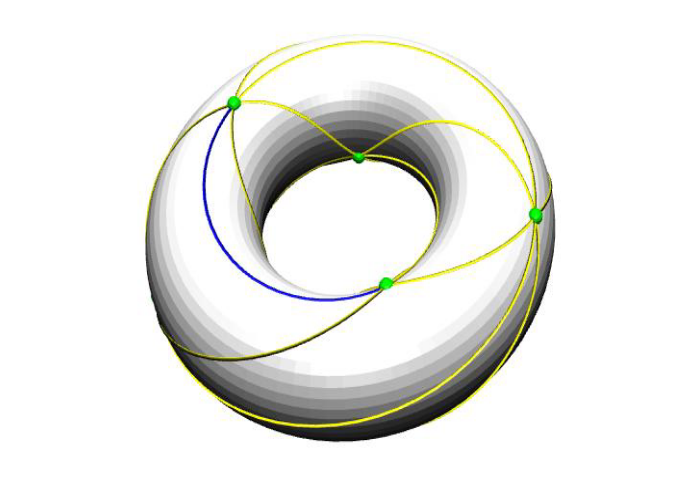
\includegraphics[width=0.5\textwidth]{img/img.png}
%     \caption{This is a caption for the image.}
%     \label{fig:image}
% \end{figure}
% Lalalala lalala

%REFERENCES
\bibliographystyle{plain}
\bibliography{bibliography.bib}

\tableofcontents

\newpage

\section{Proofs}

\subsection{Notation}
$ $\par
Let us introduce useful contractions:
\begin{align}
    &r^m_t := \nabla R(x^m_t)
    &q^m_t := \nabla Q(x^m_t)
\end{align}

Also for average values:
\begin{align}
    &\bar{r}_t := \fsumm {m=1}{M}{\nabla R(x^m_t)} \\
    &\bar{R}_t := \fsumm {m=1}{M}{R(x^m_t)} \\
    &\bar{q}_t := \fsumm {m=1}{M}{\nabla Q(x^m_t)} \overset{\text{~\ref{cor:linearity}}}{=}  \nabla Q(\bar{x}_t)
\end{align}

And for values of $Q$ and $R$ at $x_*$:
\begin{align}
    &r_* := \nabla R(x_*)
    &R_* := R(x_*) \\
    &q_* := \nabla Q(x_*)
    &Q_* := Q(x_*)
\end{align}

\subsection{Technical lemmas}

Before demonstrating the claimed facts, let's first establish some technical results.
In this section we will follow the path of proving Lemma 3.1 from \cite{Stich}.

\begin{lemma}
    \begin{align}
    \norm{\bar{x}_t - x_* - \gamma \bar{g}_t}^2
    &= \norm{\bar{x}_t - x_*}^2 
    + \gamma^2 \norm{\bar{g}_t}^2 
    - 2 \gamma \inner{\bar{x}_t - x_*}{\bar{g}_t} \\
    &= \norm{\bar{x}_t - x_*}^2 
    + \gamma^2 \norm{\bar{g}_t}^2 
    - 2 \gamma \fsumm {m=1}{M}{ \inner{\bar{x}_t - x_*}{\nabla F(x^m_t)} } \\
    &= \norm{\bar{x}_t - x_*}^2 
    + \gamma^2 \norm{\fsumm {m=1}{M}{\nabla F(x^m_t)}}^2 
    - 2 \gamma \fsumm {m=1}{M}{ \inner{\bar{x}_t - x_*}{\nabla F(x^m_t)} } \\
    &= \norm{\bar{x}_t - x_*}^2 
    + \gamma^2 \norm{\fsumm {m=1}{M}{\nabla F(x^m_t)} - \nabla F(x_*)}^2 
    - 2 \gamma \fsumm {m=1}{M}{ \inner{\bar{x}_t - x_*}{\nabla F(x^m_t)} } \\
    &= \norm{\bar{x}_t - x_*}^2 
    + \gamma^2 \norm{\fsumm {m=1}{M}{\nabla Q(x^m_t) + \nabla R(x^m_t) - \nabla Q(x_*) - \nabla R(x_*)}}^2  \\
    &- 2 \gamma \fsumm {m=1}{M}{ \inner{\bar{x}_t - x_*}{\nabla Q(x^m_t)} }
    - 2 \gamma \fsumm {m=1}{M}{ \inner{\bar{x}_t - x_*}{\nabla R(x^m_t)} }  \\
    &= \norm{\bar{x}_t - x_*}^2 
    + \gamma^2 \norm{\bar{q}_t 
    + \bar{r}_t - q_* - r_*}^2 
    - 2 \gamma \fsumm {m=1}{M}{ \inner{\bar{x}_t - x_*}{q^m_t} }
    - 2 \gamma \fsumm {m=1}{M}{ \inner{\bar{x}_t - x_*}{r^m_t} } \\
    &= \norm{\bar{x}_t - x_*}^2 
    + \gamma^2 \norm{\bar{q}_t 
    + \bar{r}_t - q_* - r_*}^2 
    - 2 \gamma \inner{\bar{x}_t - x_*}{\bar{q}_t}
    - 2 \gamma \inner{\bar{x}_t - x_*}{\bar{r}_t} \label{eq:St_0}
\end{align}
\end{lemma}


\begin{lemma} \label{lem:g_t}
    Bounding $\norm{\bar{g}_t}^2$
    \[  \norm{\bar{q}_t + \bar{r}_t - q_* - r_*}^2 \\
        \leq
        2 L_Q(1 + \zeta)  (Q(\bar{x}_t) - Q_* - \inner {q_*}{\bar{x}_t - x_*})
        + 2 L_R(1 + \frac{1}{\zeta})  (\bar{R}_t - R_* - \inner {r_*}{\bar{x}_t - x_*})
    \]
\end{lemma}
\begin{proof}
$ $\par
    By the generalized Cauchy inequality:
    \begin{align}
        &\norm{\bar{q}_t + \bar{r}_t - q_* - r_*}^2
        = \norm{\bar{q}_t - q_*}^2 
        + \norm{\bar{r}_t - r_*}^2
        + 2\inner {\bar{q}_t - q_*} {\bar{r}_t - r_*} \label{eq:St_1_1} \\
        &\leq \norm{\bar{q}_t - q_*}^2 
        + \norm{\bar{r}_t - r_*}^2 
        + \zeta \norm{\bar{q}_t - q_*}^2 
        + \frac{1}{\zeta} \norm{\bar{r}_t - r_*}^2 \label{eq:St_1_2} \\
        &= (1 + \zeta)\norm{\bar{q}_t - q_*}^2 + (1 + \frac{1}{\zeta})\norm{\bar{r}_t - r_*}^2  \label{eq:St_1_1}
    \end{align}
    
    By $L$ - smoothness and some theorem:
    \begin{align}
        (1 + \zeta)\norm{\bar{q}_t - q_*}^2 &+ (1 + \frac{1}{\zeta})\norm{\bar{r}_t - r_*}^2 \\
        &\leq 2 L_Q(1 + \zeta)  (Q(\bar{x}_t) - Q_* - \inner {q_*}{\bar{x}_t - x_*})
        + 2(1 + \frac{1}{\zeta}) L_R (\bar{R}_t - R_* - \inner {r_*}{\bar{x}_t - x_*}) \label{eq:St_1_2}
    \end{align}
    
    Combining together \eqref{eq:St_1_1} and \eqref{eq:St_1_2}, we obtain:
    \begin{align}
        \norm{\bar{q}_t + \bar{r}_t - q_* - r_*}^2 
        \leq 2 L_Q(1 + \zeta)  (Q(\bar{x}_t) - Q_* - \inner {q_*}{\bar{x}_t - x_*})
        + 2 L_R(1 + \frac{1}{\zeta})  (\bar{R}_t - R_* - \inner {r_*}{\bar{x}_t - x_*}) \label{eq:St_1}
    \end{align}
\end{proof}


\begin{lemma} \label{lem:inner_1}
    By $\mu_Q$ - convexity:
    \begin{align}
        -2 \inner{\bar{x}_t - x_*}{\bar{q}_t} &= 2 \inner{x_* - \bar{x}_t} {\bar{q}_t} \\
        &\leq 2 Q_* - 2 Q(\bar{x}_t) - \mu_Q \norm{\bar{x}_t - x_*}^2 \label{eq:St_2}
    \end{align}
\end{lemma}

\begin{lemma} \label{lem:inner_2}
\begin{align}
    \begin{split}
    - 2 \inner{\bar{x}_t - x_*}{\bar{r}_t} &\leq \\ 
     & (\bar{R}_t - R_*)(\frac{4}{p} - 2) + 2 p L_R V_t - \mu_R \norm{x_* - \bar{x}_t}^2 
     - \frac{4}{p}\inner{r_*}{\bar{x}_t - x_*}
    \end{split}
\end{align}
\end{lemma}
\begin{proof}
    \begin{align}
        - 2 \inner{\bar{x}_t - x_*}{\bar{r}_t} &= 2 \inner{x_* - \bar{x}_t} {\bar{r}_t} \\
        &= \frac{2}{M} \summ{m=1}{M}{ \inner{x_* - \bar{x}_t}{r^m_t} } 
        = \frac{2}{M} \summ{m=1}{M}{\inner{x_* - x^m_t + x^m_t - \bar{x}_t}{r^m_t}} \\
        &= \frac{2}{M} \summ{m=1}{M}{\inner{x_* - x^m_t}{r^m_t}} 
        + \frac{2}{M} \summ{m=1}{M}{\inner{x^m_t - \bar{x}_t}{r^m_t}} \label{eq:St_3_0}
    \end{align}
    
    Part one, by $\mu_R$ - convexity and Jensen's inequality:
    \begin{align}
        &\frac{2}{M} \summ{m=1}{M}{\inner{x_* - x^m_t}{r^m_t}} 
        \leq \frac{1}{M} \summ{m=1}{M}{2 R_* - 2 R(x^m_t) - \mu_R \norm{x_* - x^m_t}^2} \\
        &\leq \frac{1}{M} \summ{m=1}{M}{2 R_* - 2 R(x^m_t) - \mu_R \norm{x_* - \bar{x}_t}^2} 
        = 2 R_* - 2 \bar{R}_t - \mu_R \norm{x_* - \bar{x}_t}^2 \label{eq:St_3_1}
    \end{align}
    
    Part two, by the generalized Cauchy inequality:
    \begin{align}
        &\frac{2}{M} \summ{m=1}{M}{\inner{x^m_t - \bar{x}_t}{r^m_t}}
        = \frac{2}{M} \summ{m=1}{M}{\inner{x^m_t - \bar{x}_t}{r^m_t - r_*}} 
        + \frac{2}{M} \summ{m=1}{M}{\inner{x^m_t - \bar{x}_t}{r_*}} \\
        &= \frac{2}{M} \summ{m=1}{M}{\inner{x^m_t - \bar{x}_t}{r^m_t - r_*}} 
        \leq \frac{2}{M} \summ{m=1}{M}{p L_R \norm{x^m_t - \bar{x}_t}^2 }
        + \frac{2}{M} \summ{m=1}{M}{\frac{1}{p L_R} \norm{r^m_t-r_*}^2 } \\
        &= 2 p L_R V_t 
        + \frac{2}{M} \summ{m=1}{M}{\frac{1}{p L_R} \norm{r^m_t-r_*}^2 } \label{eq:St_3_2_1}
    \end{align}
    
    By some theorem:
    \begin{align}
        \norm{r^m_t-r_*}^2 \leq 2L_R (R(x^m_t) - R_* - \inner {r_*}{x^m_t - x_*}) \label{eq:St_3_2_2}
    \end{align}
    
    Substituting \eqref{eq:St_3_2_2} into \eqref{eq:St_3_2_1}, we complete part two:
    \begin{align}
        &\frac{2}{M} \summ{m=1}{M}{\inner{x^m_t - \bar{x}_t}{r^m_t}}
        \leq 2 p L_R V_t 
        + \frac{4}{pM} \summ{m=1}{M}{R(x^m_t) - R_* - \inner {r_*}{x^m_t - x_*} } \\
        &\leq 2 p L_R V_t 
        + \frac{4}{p} (\bar{R}_t - R_* - \inner {r_*}{\bar{x}_t - x_*}) \label{eq:St_3_2}
    \end{align}
    
    Combining together \eqref{eq:St_3_0}, \eqref{eq:St_3_1}, \eqref{eq:St_3_2}, we gain:
    \begin{align}
         - 2 \inner{\bar{x}_t - x_*}{\bar{r}_t} &\leq
         2 R_* - 2 \bar{R}_t - \mu_R \norm{x_* - \bar{x}_t}^2 
         + 2 p L_R V_t + \frac{4}{p} (\bar{R}_t - R_* - \inner {r_*}{\bar{x}_t - x_*}) \\ 
         &= (\bar{R}_t - R_*)(\frac{4}{p} - 2) + 2 p L_R V_t - \mu_R \norm{x_* - \bar{x}_t}^2 
         - \frac{4}{p}\inner{r_*}{\bar{x}_t - x_*}
         \label{eq:St_3}
    \end{align}
\end{proof}

\begin{lemma}\label{lem:AB-lemma}
    \begin{align}
    \begin{split}
        &\norm{\bar{x}_t - x_* - \gamma \bar{g}_t}^2 \leq \\
        &(1 - \gamma \mu)\norm{\bar{x}_t - x_*}^2 + 2 \gamma p L_R V_t \\
        &+ 2\gamma (A - 1)(Q(\bar{x}_t) - Q_*) \\
        &+ 2\gamma (B - 1)(\bar{R}_t - R_*) \\
        &- 2\gamma A \inner{q_*}{\bar{x}_t - x_*} \\
        &- 2\gamma B \inner{r_*}{\bar{x}_t - x_*}
    \end{split}
\end{align}
Where $A$ and $B$ are functions of $\zeta$ such that:
\[A = \gamma L_Q(1+\zeta)\] \[B = \gamma L_R(1+\frac{1}{\zeta}) + \frac{2}{p}\]

\end{lemma}
\begin{proof} Substituting the results of Lemmas~\ref{lem:g_t},~\ref{lem:inner_1} and~\ref{lem:inner_2} into \eqref{eq:St_0} and doing some algebraic manipulations:
    \begin{align}
        \begin{split}
            &\norm{\bar{x}_t - x_* - \gamma \bar{g}_t}^2 \leq \norm{\bar{x}_t - x_*}^2 \\
            &+ 2\gamma^2 L_Q (1 + \zeta) (Q(\bar{x}_t) - Q_* - \inner {q_*}{\bar{x}_t - x_*}) \\
            &+ 2\gamma^2 L_R (1 + \frac{1}{\zeta}) (\bar{R}_t - R_* - \inner {r_*}{\bar{x}_t - x_*}) \\
            &+ \gamma ( 2 Q_* - 2 Q(\bar{x}_t) - \mu_Q \norm{\bar{x}_t - x_*}^2 ) \\
            &+ \gamma(\bar{R}_t - R_*)(\frac{4}{p} - 2) + 2 \gamma p L_R V_t - \gamma \mu_R \norm{x_* - \bar{x}_t}^2 - \frac{4}{p}\inner{r_*}{\bar{x}_t - x_*}\\
            &= (1 - \gamma \mu_Q - \gamma \mu_R)\norm{\bar{x}_t - x_*}^2 + 2 \gamma p L_R V_t \\
            &+ (Q(\bar{x}_t) - Q_*)\coef {2\gamma^2 L_Q (1+\zeta) - 2\gamma}
            + (\bar{R}_t - R_*)\coef{2\gamma^2 L_R (1+\frac{1}{\zeta}) - 2\gamma + \frac{4\gamma}{p}} \\
            &- 2\inner{q_*}{\bar{x}_t - x_*}\coef{\gamma^2 L_Q(1+\zeta)}
            - 2\inner{r_*}{\bar{x}_t - x_*}\coef{\gamma^2 L_R(1+\frac{1}{\zeta}) + \frac{2\gamma}{p}} \label{eq:lol}
        \end{split}
    \end{align}
    Using the result of Lemma~\ref{lem:mu-lemma}:
    \begin{align}
        (1 - \gamma \mu_Q - \gamma \mu_R)\norm{\bar{x}_t - x_*}^2 \leq (1 - \gamma \mu)\norm{\bar{x}_t - x_*}^2 \label{eq:mu-eq}
    \end{align}
    Combining \eqref{eq:mu-eq} with \eqref{eq:lol}
    \begin{align}
        \begin{split}
             &\norm{\bar{x}_t - x_* - \gamma \bar{g}_t}^2 \leq 
            (1 - \gamma \mu)\norm{\bar{x}_t - x_*}^2 + 2 \gamma p L_R V_t \\
            &+ (Q(\bar{x}_t) - Q_*)\coef {2\gamma^2 L_Q (1+\zeta) - 2\gamma}
            + (\bar{R}_t - R_*)\coef{2\gamma^2 L_R (1+\frac{1}{\zeta}) - 2\gamma + \frac{4\gamma}{p}} \\
            &- 2\inner{q_*}{\bar{x}_t - x_*}\coef{\gamma^2 L_Q(1+\zeta)}
            - 2\inner{r_*}{\bar{x}_t - x_*}\coef{\gamma^2 L_R(1+\frac{1}{\zeta}) + \frac{2\gamma}{p}} \\
            &= (1 - \gamma \mu)\norm{\bar{x}_t - x_*}^2 + 2 \gamma p L_R V_t \\
            &+ 2\gamma (Q(\bar{x}_t) - Q_*)\coef{\gamma L_Q (1+\zeta) - 1)} 
            + 2\gamma (\bar{R}_t - R_*)\coef{\gamma L_R (1+\frac{1}{\zeta}) - 1 + \frac{2}{p}} \\
            &- 2\gamma \inner{q_*}{\bar{x}_t - x_*}\coef{\gamma L_Q(1+\zeta) }
            - 2\gamma \inner{r_*}{\bar{x}_t - x_*}\coef{\gamma L_R(1+\frac{1}{\zeta}) + \frac{2}{p}}
        \end{split}
    \end{align}
        
By substituting the expressions in square brackets with $A$ and $B$, we obtain the statement of the lemma.
\end{proof}

\begin{lemma}\label{lem:Technical}
    Exists $\zeta_1$ such that $A(\zeta_1) = B(\zeta_1)$ and $A(\zeta_1) - 1 \leq 0$
\end{lemma}
\begin{sublemma}\label{sublem:sublemma_1}
    Exists $\zeta_1$ such that $A(\zeta_1) = B(\zeta_1)$
\end{sublemma}
\begin{proof}
    By equating $A$ and $B$, we obtain the chain of equalities:

    \begin{align}
        &\gamma L_Q(1+\zeta)= \gamma L_R(1+\frac{1}{\zeta}) + \frac{2}{p} \\
        &L_Q(1+\zeta) = L_R(1+\frac{1}{\zeta}) + \frac{2}{\gamma p} \\
        &L_Q + \zeta L_Q - L_R - \frac{L_R}{\zeta} - \frac{2}{\gamma p} = 0 \\
        &\zeta L_Q + \zeta^2 L_Q - \zeta L_R - L_R - \frac{2\zeta}{\gamma p} \\
        &\zeta^2 L_Q + \zeta (L_Q - L_R - \frac{2}{\gamma p}) - L_R = 0 \\
        &\zeta_{1} := \frac{-(L_Q - L_R - \frac{2}{\gamma p}) + \sqrt{(L_Q - L_R - \frac{2}{\gamma p})^2 + 4 L_Q L_R}}{2L_Q} > 0
    \end{align}
    
    Hence,
    \begin{align}
        \gamma L_R (1+\frac{1}{\zeta_1}) + \frac{2}{p} = \gamma L_Q (1+\zeta_1) \label{eq:St_5}
    \end{align}
\end{proof}


\begin{sublemma}\label{sublem:sublemma_2}
    For $\zeta_1$ from previous lemma: $A(\zeta_1) - 1 \leq -\frac{1}{10} \leq 0$
\end{sublemma}
\begin{proof}
    $\gamma \leq \frac{1}{6 L}$, meaning that $L \leq \frac{1}{6 \gamma }$:
    \begin{align}
        A(\zeta_1)& - 1 = \gamma L_Q(1+\zeta_1) - 1 \\
        &= \gamma L_Q 
        \coef {1 + \frac{-(L_Q - L_R - \frac{2}{\gamma p})+\sqrt{(L_Q - L_R -\frac{2}{\gamma p})^2 + 4 L_Q L_R}}{2L_Q} } - 1\\
        &=
        \frac{\gamma}{2} 
        \coef {2L_Q - (L_Q - L_R - \frac{2}{\gamma p}) + \sqrt{(L_Q - L_R - \frac{2}{\gamma p})^2 + 4 L_Q L_R} } - 1\\ 
        & \leq
        \frac{\gamma}{2} 
        \coef {|L_Q + L_R + \frac{2}{\gamma p}| + |L_Q - L_R - \frac{2}{\gamma p}| + \sqrt{ 4 L_Q L_R} } - 1\\
        & \leq
        \frac{\gamma}{2} 
        \coef {L_Q + L_R + \frac{2}{\gamma p} + L_Q + L_R + \frac{2}{\gamma p} + \sqrt{ 4 L^2} } - 1\\
        & \leq
        \frac{\gamma}{2} 
        \coef {6 L + \frac{4}{\gamma p} } - 1
        \leq
        \frac{\gamma}{2} 
        \coef {\frac{6}{6 \gamma} + \frac{4}{\gamma p} } - 1 \\
        &=
        \frac{1}{2} + \frac{2}{p} - 1
        = \frac{2}{p} - \frac{1}{2}
    \end{align}
    
    For $p \geq 5$:
    \begin{align}
         \gamma L_Q(&1+\zeta_1) - 1 \leq \frac{2}{p} - \frac{1}{2} \leq \frac{2}{5} - \frac{1}{2} 
         = -\frac{1}{10} < 0 \label{eq:St_6}
    \end{align}
\end{proof}

Combining the results of Sublemmas~\ref{sublem:sublemma_1} and~\ref{sublem:sublemma_2}, 
we obtain the statement of Lemma ~\ref{lem:Technical}.



Further, let's denote $A_1$ as $A(\zeta_1)$ and $B_1$ as $B(\zeta_1)$
\begin{lemma} \label{lem:main}
    \begin{align}
        \begin{split}
            \norm{\bar{x}_t - x_* - \gamma \bar{g}_t}^2 \leq (1 - \gamma \mu)\norm{\bar{x}_t - x_*}^2  + 10 \gamma L_R V_t
        \end{split}
    \end{align}
\end{lemma}
\begin{proof}
    From Lemma~\ref{lem:AB-lemma} we know that:
    \begin{align}
        \begin{split}
            \norm{\bar{x}_t - x_* - \gamma \bar{g}_t}^2 \leq \\
            &(1 - \gamma \mu)\norm{\bar{x}_t - x_*}^2 + 2 \gamma p L_R V_t \\
            &+ 2\gamma (A - 1)(Q(\bar{x}_t) - Q_*)
            + 2\gamma (B - 1)(\bar{R}_t - R_*) \\
            &- 2\gamma A \inner{q_*}{\bar{x}_t - x_*}
            - 2\gamma B \inner{r_*}{\bar{x}_t - x_*} \label{eq:main}
        \end{split}
    \end{align}
    Using the result of Lemma~\ref{lem:Technical}, and substituting $\zeta_1$ into $A$ and $B$, we obtain that $A = B = A_1 = B_1$:
    \begin{align}
        - 2\gamma A_1 \inner{q_*}{\bar{x}_t - x_*} - 2\gamma B_1 \inner{r_*}{\bar{x}_t - x_*} 
        &= - 2\gamma A_1 \inner{q_* + r_*}{\bar{x}_t - x_*} \\
        &= - 2\gamma A_1 \inner{\nabla F(x_*)}{\bar{x}_t - x_*} = 0 \label{eq:zero}
    \end{align}

    For $a \geq 0$ by Jensen's inequality:
    \begin{align}
        -a (\fsumm{m=1}{M}{R(x^m_t}) - R_*) \leq -a (R(\bar{x}_t) - R_*) \label{eq:jensen'} 
    \end{align}
    
    Using that $A_1 - 1 \leq 0$ allows us to use \eqref{eq:jensen'}:
    \begin{align}
        2\gamma (B_1 - 1)(\bar{R}_t - R_*) &= 2\gamma (A_1 - 1)(\bar{R}_t - R_*) \\
        &= |2\gamma (A_1 - 1)| \cdot (R_* - \bar{R}_t) = |2\gamma (A_1 - 1)| \cdot (R_* - \fsumm{m=1}{M}{R(x^m_t})) \\
        &\leq |2\gamma (A_1 - 1)| \cdot (R_* - R(\bar{x}_t)) = 2\gamma (A_1 - 1) (R(\bar{x}_t) - R_*) \label{eq:jensen}
    \end{align}
    Substituting \eqref{eq:zero} and \eqref{eq:jensen} into \eqref{eq:main}:
    \begin{align}
        &\norm{\bar{x}_t - x_* - \gamma \bar{g}_t}^2 \\
        &\leq (1 - \gamma \mu)\norm{\bar{x}_t - x_*}^2 + 2 \gamma p L_R V_t
        + 2\gamma (A_1 - 1)(Q(\bar{x}_t - Q_* + R(\bar{x}_t - R_*) \\
        &= (1 - \gamma \mu)\norm{\bar{x}_t - x_*}^2 + 2 \gamma p L_R V_t
        + 2\gamma (A_1 - 1)(F(\bar{x}_t - F_*)
    \end{align}
    Given that Lemma~\ref{lem:Technical} holds for $p = 5$ and utilizing the fact that $F(\bar{x}t) - F* \geq 0$:
    \begin{align}
        \norm{\bar{x}_t - x_* - \gamma \bar{g}_t}^2 &
        \leq (1 - \gamma \mu)\norm{\bar{x}_t - x_*}^2 + 10 \gamma L_R V_t
        + 2\gamma (A_1 - 1)(F(\bar{x}_t - F_*) \\
        &\leq (1 - \gamma \mu)\norm{\bar{x}_t - x_*}^2 + 10 \gamma L_R V_t
    \end{align}
    Thus completing the proof.
\end{proof}

\subsection{Other Lemmas}
\begin{lemma} \label{lem:var_red}
    Variance reduction:
    \begin{align}
        \E \norm{g_t - \bar{g}_t}^2 \leq \frac{\sigma^2}{M}
    \end{align}
\end{lemma}
\begin{proof} This is Lemma 3.2 in \cite{Stich}. By independence of $g^m_t$ on each device:
    \begin{align}
        \E \norm{g_t - \bar{g}_t}^2 \leq \E \norm{\fsumm{m=1}{M}{g^m_t - \bar{g}^m_t}}^2 
        = \fsumm{m=1}{M} \E \norm{g^m_t - \bar{g}^m_t}^2 \leq \frac{\sigma^2}{M}
    \end{align}
\end{proof}

\begin{lemma} \label{lem:lemma_Vt}
    \begin{align}
        \E [V_t] \leq (H-1) \gamma^2 \sigma^2
    \end{align}
\end{lemma}
\begin{proof}
    This is Lemma 1 in \cite{Khaled}.
\end{proof}

\subsection{Proof of Theorem~\ref{th:th_1}}
\begin{proof}
    Consider $\gamma \leq \frac{1}{6L}$ and $\mu > 0$.
    Using the update equation \eqref{eq:upd_eq} we have
    \begin{align}
        \norm{\bar{x}_{t+1}-x_*}^2
        &= \norm{\bar{x}_{t} - \gamma g_t - x_*}^2
        = \norm{\bar{x}_{t} - \gamma g_t - x_* - \gamma \bar{g}_t + \gamma \bar{g}_t}^2 \\
        &= \norm{\bar{x}_t - x_* - \gamma \bar{g}_t}^2 
        + \gamma^2 \norm{g_t - \bar{g}_t}^2
        + 2 \gamma \inner{\bar{x}_t - x_* - \gamma \bar{g}_t}{g_t - \bar{g}_t}
    \end{align}
    
    Taking expectation, 
    \begin{align}
        \E \norm{\bar{x}_{t+1}-x_*}^2
        &= \E \norm{\bar{x}_t - x_* - \gamma \bar{g}_t}^2
        + \gamma^2 \E \norm{g_t - \bar{g}_t}^2 \label{eq:eq81}
    \end{align}
    
    
    Taking expectiation of result of Lemma~\ref{lem:main}:
    \begin{align}
        \E \norm{\bar{x}_t - x_* - \gamma \bar{g}_t}^2 
        \leq (1 - \gamma \mu) \E \norm{\bar{x}_t - x_*}^2 + 10 \gamma L_R \E [V_t] \label{eq:eq82}
    \end{align}

    Combining \eqref{eq:eq81}, \eqref{eq:eq82} with Lemma~\ref{lem:lemma_Vt} and Lemma~\ref{lem:var_red}
    \begin{align}
         \E \norm{\bar{x}_{t+1}-x_*}^2
        &\leq (1 - \gamma \mu) \E \norm{\bar{x}_t - x_*}^2 
        + \gamma^2 \E \norm{g_t - \bar{g}_t}^2
        + 10 \gamma L_R \E [V_t] \\
        &\leq
        (1 - \gamma \mu) \E \norm{\bar{x}_t - x_*}^2 
        + \frac{\gamma^2 \sigma^2}{M}
        + 10 \gamma L_R (H-1) \gamma^2 \sigma^2 \label{eq:eq83}
    \end{align}

    Recursing \eqref{eq:eq83}, we obtain
    \begin{align}
        \E \norm{\bar{x}_{T}-x_*}^2 
        & \leq (1 - \gamma \mu)^T \E \norm{\bar{x}_0 - x_*}^2 
        + \frac{\gamma \sigma^2} {\mu M} 
        + \frac{10 L_R (H-1) \gamma^2 \sigma^2}{\mu}
    \end{align}

    It remains to notice that by assumtion~\ref{ass:ass_3} we have $L_R = \varepsilon L$.
\end{proof}

\subsection{Proof of Theorem~\ref{th:th_2}}


\end{document}
